\section{Firmware Design and Implementation}

This section presents the firmware development for the STM32U5-microcontroller~\cite{stm32u5}, which forms the core of the low-energy backup communication system.
The firmware is responsible for real-time handling of LoRa communication, sensor data processing, and voice output via speech synthesis or WAV file playback. 
To achieve real-time performance, the firmware is built on FreeRTOS~\cite{freertos}, as illustraded in Figure-\ref{fig:firmware-system}. This enables clear separation of tasks with different priorities, making development more structured and maintainable.

\begin{figure}[H]
\centering
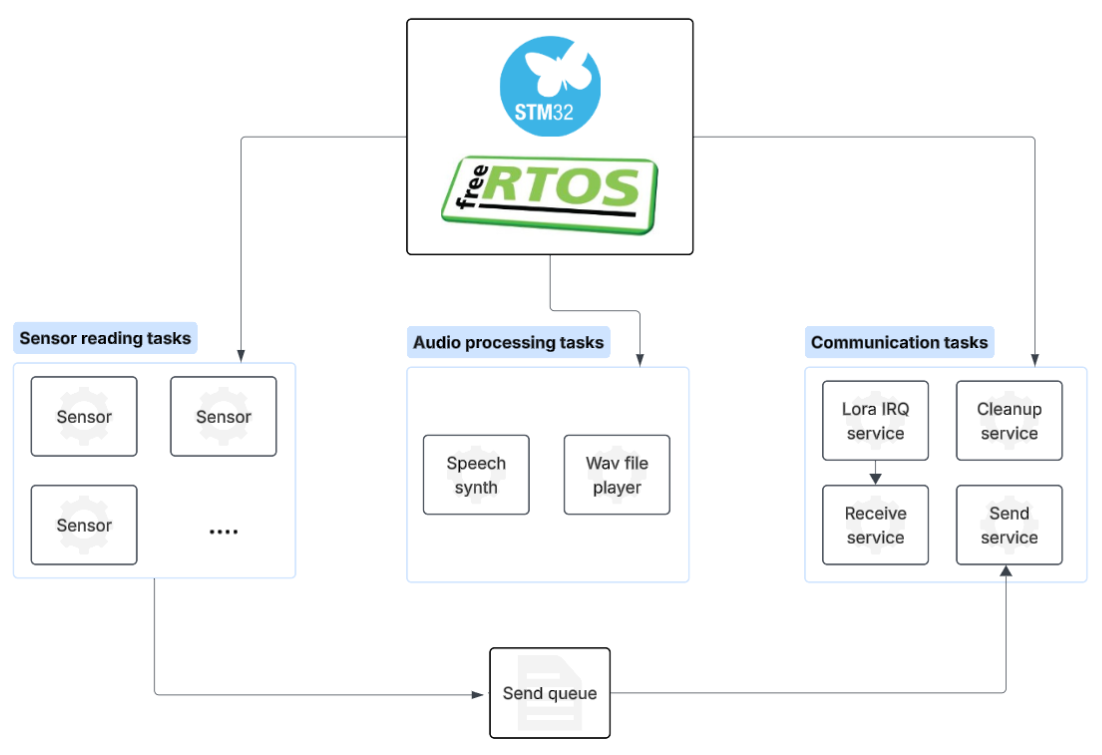
\includegraphics[width=0.45\textwidth]{images/firmware-system-design.png}
\caption{Firmware system architecture overview}\label{fig:firmware-system}
\end{figure}

\subsection{Firmware Architecture}

As seen on Figure-\ref{fig:firmware-system}, the architecture is organized into three different modules which use inter-task communication mechanisms provided by FreeRTOS. 

\paragraph{LoRa Communiction Group}

This group consists of four different tasks: \textit{Receive}, \textit{Send}, \textit{IRQ Handling} and \textit{Cleanup}. The Recieve task blocks on a semaphore that will be set when the IRQ handling task get interupted by the sx1276-module~\cite{sx1276}, to notfiy receive/transmit completion.


\paragraph{Sensor Management Group}

\paragraph{Audio Processing Group}

\paragraph{Power and Memory Management}

% What i want to say:
%  - Heap-5 memory section in upper region of ram -> making disabling of ram blocks more straight forward
%  - System architecture consisting of, 
%     LoRa Communiction group: receiving (waiting or IRQ task), sending (Waiting for message to send), cleanup (Periodic cleanup of heap allocated objects)
%     Sensor group: Multiple sensor task using send queue to send data over LoRa
%     Audio group: Ported espeak-ng to embedded system by removing file system references and hardcoding values, wav-file playback by converting wav files to c-arrays.
% 
%  - LoRa Hardware accelerated AES in CTR mode
%  - 
% 

